\begin{figure*}[t]
\centering
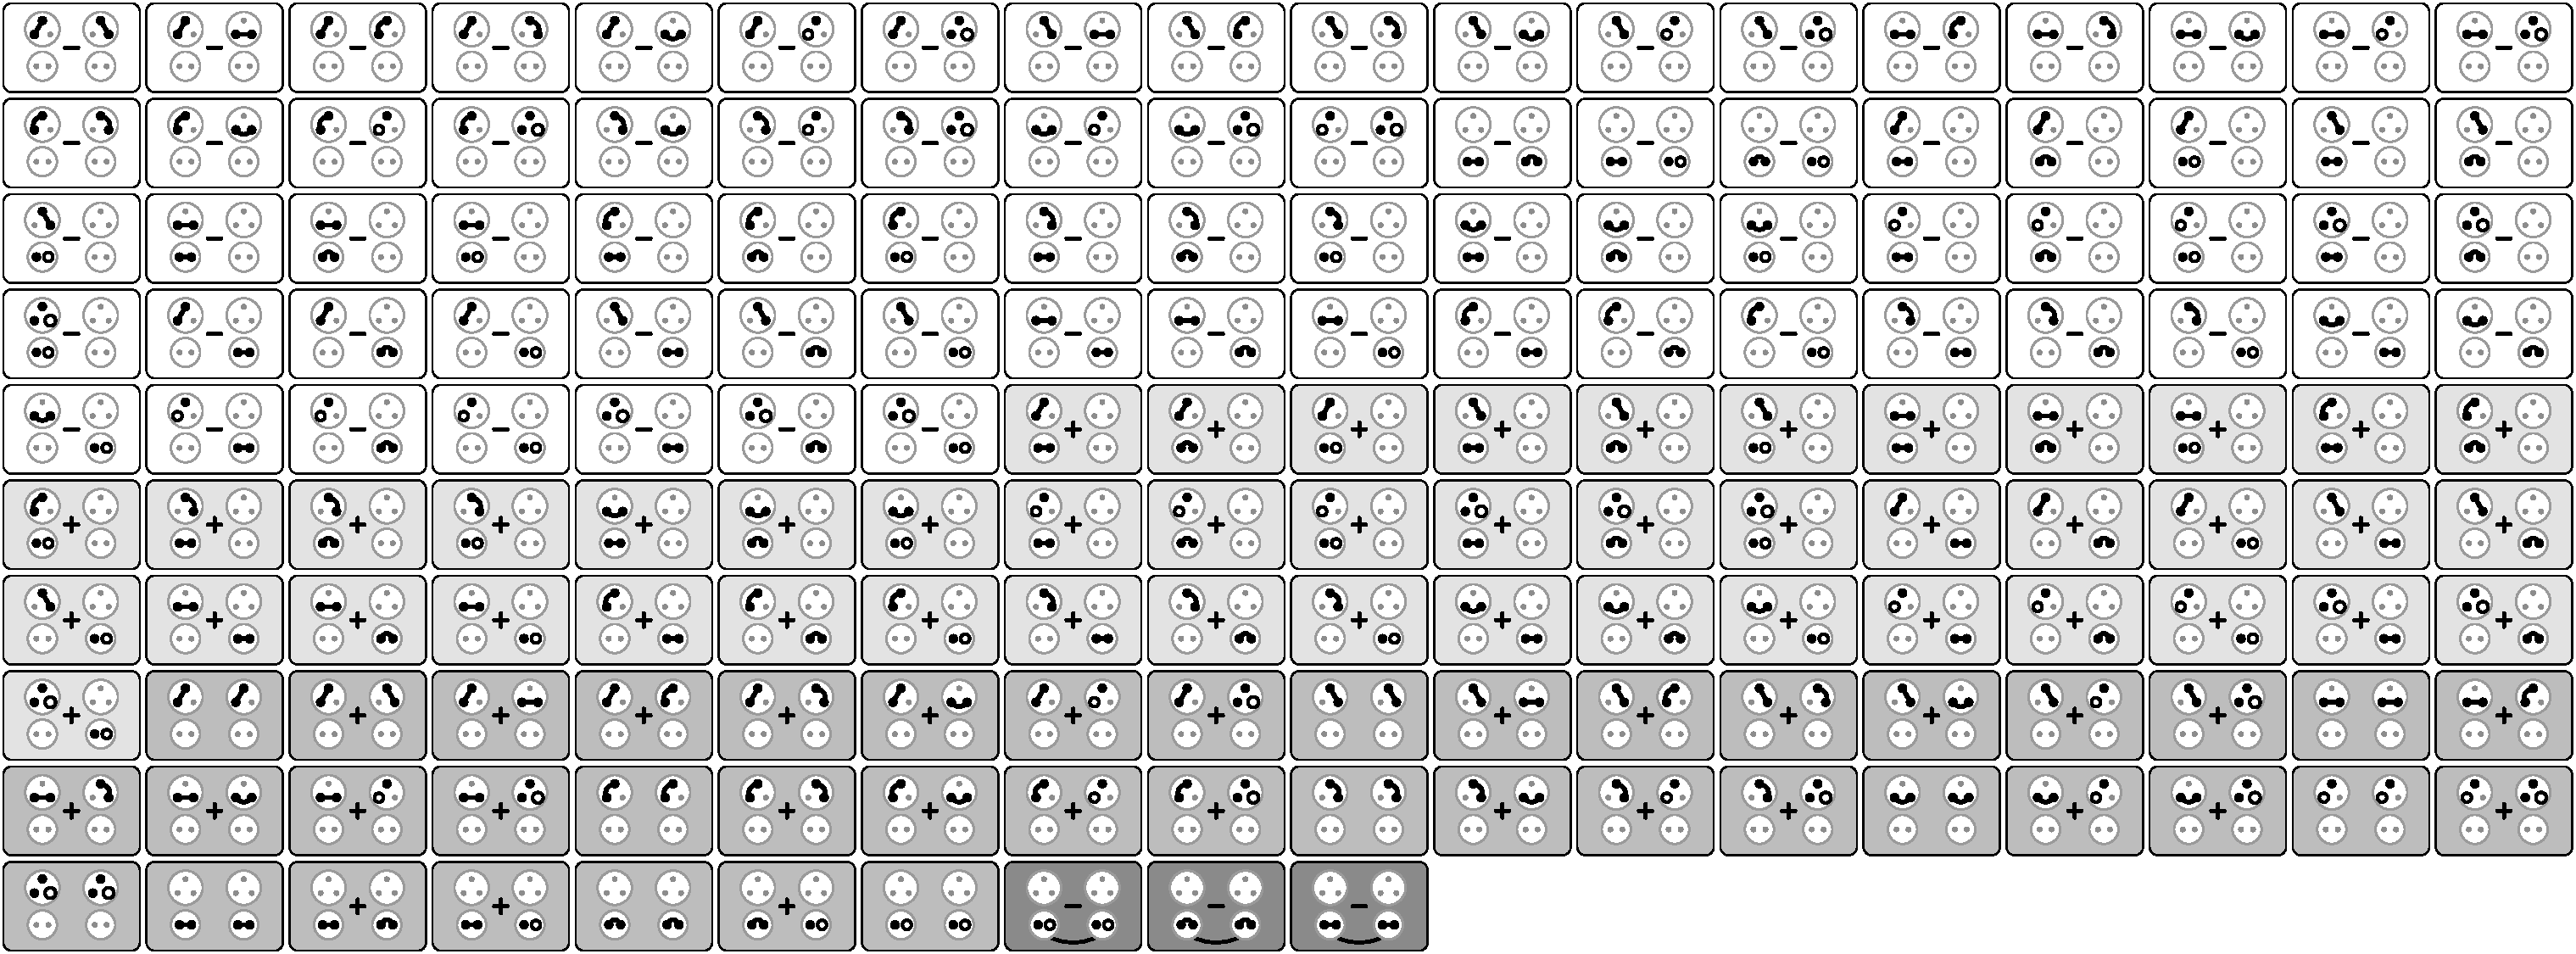
\includegraphics[width=\textwidth]{figures/records_atlas.pdf}
\caption{The $172$ measurement records of the object, one drawing each, on the square of slots of Fig.~\ref{fig:link}(b), with the qutrit copies $Q_{1}$, $Q_{2}$ above, with three dots, the basis directions, and the read qubits $q_{1}$, $q_{2}$ below, with two. Each record's two letters are drawn in their slots. A straight line joining two dots is a symmetric off-diagonal letter, a curved line an antisymmetric one, and filled and hollow dots a diagonal one. A $+$ or $-$ marks a record that is the drawing plus or minus its image under the exchange of the reads; a drawing with no sign is its own image. The three cells with an arc under the qubits are the commutator records, in which each qubit shows the commutator of two qubit letters, itself a single letter, and the record is the commutator at $q_{1}$ minus the same at $q_{2}$. Each cell's shade gives its weight $\sqrt{k_{r}}$ of Eq.~(\ref{eq:gain}), white for the $79$ records at $1$, light and then mid gray for the $48$ at $\sqrt{2}$ and the $42$ at $\sqrt{3}$, and dark gray for the $3$ at $\sqrt{6}$, the sectors of Table~\ref{tab:sectors}; the cells are sorted by weight. The drawings depend on the choice of basis; the counts and weights do not. The figure is drawn from the construction of the ancillary record script~\cite{SM}.}
\label{fig:records}
\end{figure*}
